%!TEX encoding = UTF-8 Unicode
%!TEX root = ../compendium2.tex

\chapter{Kojo}\label{appendix:kojo}

\section{Vad är Kojo?}

Kojo%
\footnote{\href{https://en.wikipedia.org/wiki/Kojo_(programming_language)}{en.wikipedia.org/wiki/Kojo\_(programming\_language)}}
 är en integrerad utvecklingsmiljö för Scala som är speciellt anpassad för programmeringsundervisning i grundskolan. Kojo används i LTH:s Science Center Vattenhallen för utbildning av grundskolelärare i programmering och vid skolbesök och annan besöksverksamhet, i vilken lärare och studenter vid LTH arbetar som handledare. 
 
 Kojo är öppen källkod och utvecklingsgemenskapen leds av Lalit Pant från Indien. I Kojo finns även lättillgängliga bibliotek som gör tröskeln lägre att programmera rörlig grafik och enkla spel.

Under kursens första laboration använder vi grafikbiblioteket i Kojo för att illustrera grundläggande begrepp, så som sekvens, alternativ, repetition och abstraktion.  


\begin{figure}[H]
\centering
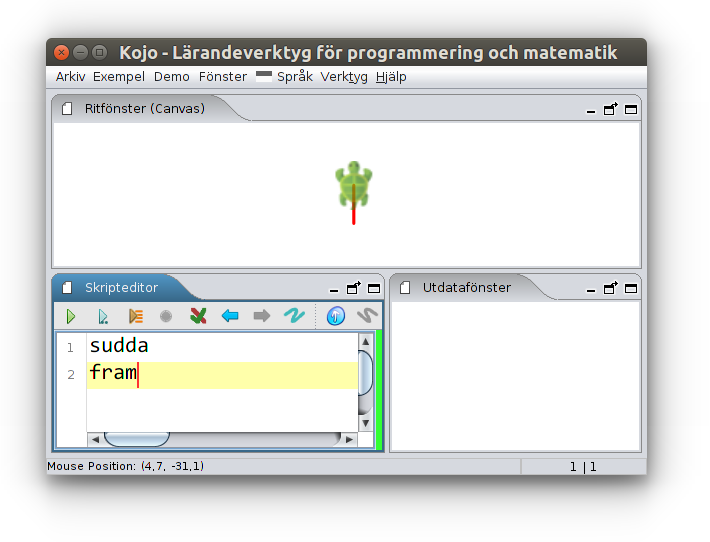
\includegraphics[width=0.8\textwidth]{../img/kojo/kojo.png}
\caption{Den nybörjarvänliga utvecklingsmiljön Kojo för Scala på svenska.}
\label{fig:appendix:ide:kojo}
\end{figure}

\section{Använda grafikbiblioteket i Kojo}\label{appendix:ide:kojo:install}

Kojo bygger på den beprövade pedagogiska idén med sköldpaddsgrafik \Eng{turtle graphics}\footnote{\url{https://en.wikipedia.org/wiki/Turtle_graphics}}, där du skriver program som styr en sköldpadda med en penna under magen. När sköldpaddan rör sig bildas ett streck av valfri färg på skärmen. Beroende på hur du bestämmer att sköldpaddan ska röra sig och vilken färg du bestämmer att pennan ska ha, kan du skapa olika intressanta bilder och samtidigt lära dig om programmeringens grunder.

Under kursens första laboration ska du använda grafikbiblioteket i Kojo tillsammans med editorn VS \code{code} och \code{scala-cli} i terminalen (se appendix \ref{appendix:terminal} och \ref{appendix:compile}). Ladda ner filen \texttt{kojo.scala} från \url{https://cs.lth.se/pgk/kojolib} och spara i en ny katalog med hjälp av din webbläsare, eller via dessa kommandon:

\begin{REPLnonum}
> mkdir w01-kojo
> cd w01-kojo
> curl -o kojolib.scala -sL https://cs.lth.se/pgk/kojolib
\end{REPLnonum}

Nu kan du starta Scala REPL och rita med Kojo så här:

\begin{REPLnonum}
> scala-cli repl .
Welcome to Scala 3.1.2 (17.0.2, Java OpenJDK 64-Bit Server VM).
Type in expressions for evaluation. Or try :help.
                                                                                                                               
scala> fram; höger; fram; vänster

\end{REPLnonum}

Du kan starta VS \code{code} i aktuellt bibliotek så här:
\begin{REPLnonum}
> code .
\end{REPLnonum}

Skriv nedan progam i VS \code{code} och spara det i samma katalog som den tidigare nedladdade filen, under ett nytt valfritt filnamn, t.ex. \code{rita.scala}:

\begin{Code}
@main def rita = fram; höger; fram; vänster
\end{Code}

Kör ditt fristående program med:
\begin{REPLnonum}
> scala-cli run .
\end{REPLnonum}

Du ska nu få upp ett fönster som heter Kojo Canvas med en sköldpadda som ritat två streck. När du stänger fönstret så avslutas programmet. Prova fler sköldpaddsfunktioner enligt tabell \ref{table:kojo:functions}.

I stället för att ladda ned filen \code{kojolib.scala} så kan du placera dess innehåll på lämpligt ställe i ditt program enligt nedan. Observera att raden som börjar med \code{//> using lib} ska vara en enda lång rad utan radbrytningar.%\code{export} gör Kojos kommandon tillgängliga utan prefix:
\lstinputlisting[breaklines=true,basicstyle=\ttfamily\fontsize{9}{11}\selectfont]{../workspace/w01_kojo/kojo.scala}

\noindent Scala-koden för den svenska paddans api finns här: \\
%\href{https://github.com/litan/kojo/blob/master/src/main/scala/net/kogics/kojo/lite/i18n/svInit.scala}{github.com/litan/kojo/blob/master/src/main/scala/net/kogics/kojo/lite/i18n/svInit.scala} \\
\href{https://github.com/litan/kojo-lib/blob/main/src/main/scala/net/kogics/kojo/i18n/Swedish.scala}{github.com/litan/kojo-lib/blob/main/src/main/scala/net/kogics/kojo/i18n/Swedish.scala}


%Kojo kräver (numera) \emph{inte} att \texttt{java} finns på din dator utan kommer med en egen JVM. 
%Eftersom du behöver tillgång till JDK i kursen, är det lika bra att installera hela JDK direkt (och inte bara JRE, så som beskrivs å länken ovan); se vidare hur du gör detta i avsnitt \ref{appendix:compile:install-jdk}.
%\href{http://www.kogics.net/kojo-download}{www.kogics.net/kojo-download}



\section{Kojo Desktop}

Kojo finns som fristående skrivbordsapplikation, kallad Kojo Desktop. Kojo Desktop innehåller en egen editor med syntaxfärgning för Scala, men fungerar ännu så länge bara för Scala 2. En av de synligaste skillnaderna mellan Scala 2 och Scala 3 är att klammerparenteser vid flerradiga funktioner är nödvändiga i Scala 2, medan Scala 3 har valfria klammerparenteser. Så om du använder Kojo Desktop behöver du komma ihåg att omgärda sekvenser av rader som hör ihop med \code|{| och \code|}|. 

Kojo Desktop är förinstallerad på LTH:s datorer och körs igång med terminalkommandot \texttt{kojo} eller via applikationsmenyn.  För instruktioner om hur du installerar Kojo Desktop på din egen dator se här: \href{http://www.lth.se/programmera/installera/}{lth.se/programmera/installera}

När du startar Kojo första gången, välj ''Svenska'' i språkmenyn och starta om Kojo. Därefter fungerar grafikfunktionerna på svenska enligt tabell \ref{table:kojo:functions} på sidan \pageref{table:kojo:functions}. När du startat om Kojo inställt på svenska ser programmet ut ungefär som i figur \ref{fig:appendix:ide:kojo} på sidan \pageref{fig:appendix:ide:kojo}.

Det finns ett antal användbara kortkommando som du hittar i menyerna i Kojo Desktop. Undersök speciellt Ctrl+Alt+Mellanslag som ger autokomplettering baserat på det du börjat skriva.

\section{Kojo i Webbläsaren}

En begränsad variant av Kojo finns tillgänglig för programmering direkt i din webbläsare här: \url{http://kojo.lu.se/}

När du trycker på play-knappen så kompileras din kod på en server till Javascript via ScalaJS och därefter körs Javascript-koden i din webbläsare. 
Kojo på webben är också ännu så länge begränsad till Scala 2 och kräver att du omgärdar sekvenser av rader som hör ihop med \code|{| och \code|}|.


\section{Mer om Kojo}

I detta dokument finns en enkel introduktion till Kojo: \\ ''Introduction to Kojo'' \url{http://www.kogics.net/kojo-ebooks#intro}

\noindent I tabell \ref{table:kojo:functions}, som fortsätter på efterföljande sidor, finns ett urval av kommando i Kojo på svenska och engelska.

{\small\renewcommand{\arraystretch}{1.4}
\begin{longtable}{@{}p{0.42\textwidth} p{0.55\textwidth}}

\caption{Ett urval av funktioner i Kojo. Se även \href{http://lth.se/programmera}{lth.se/programmera}}\label{table:kojo:functions}\\

\emph{Svenska/Engelska} & \emph{Vad händer?}  \\ \hline
\code|sudda| \newline \code|clear| & Ritfönstret suddas \\
\code|fram| \newline \code|forward()| & Paddan går framåt 25 steg. \\
\code|fram(100)| \newline \code|forward(100)| & Paddan går framåt 100 steg. \\
\code|höger| \newline \code|right(90)| & Paddan vrider sig 90 grader åt höger. \\
\code|höger(45)| \newline \code|right(45)| & Paddan vrider sig 45 grader åt höger. \\
\code|vänster| \newline \code|left(90)| & Paddan vrider sig 90 grader åt vänster. \\
\code|vänster(45)| \newline \code|left(45)| & Paddan vrider sig 45 grader åt vänster. \\
\code|hoppa| \newline \code|hop| & Paddan hoppar 25 steg utan att rita. \\
\code|hoppa(100)| \newline \code|hop(100)| & Paddan hoppar 100 steg utan att rita. \\
\code|hoppaTill(100, 200)| \newline \code|jumpTo(100, 200)| & Paddan hoppar till läget (100, 200) utan att rita. \\
\code|gåTill(100, 200)| \newline \code|moveTo(100, 200)| & Paddan vrider sig och går till läget (100, 200). \\
\code|hem| \newline \code|home| & Paddan går tillbaka till utgångsläget (0, 0). \\
\code|öster| \newline \code|setHeading(0)| & Paddan vrider sig så att nosen pekar åt höger. \\
\code|väster| \newline \code|setHeading(180)| & Paddan vrider sig så att nosen pekar åt vänster. \\
\code|norr| \newline \code|setHeading(90)| & Paddan vrider sig så att nosen pekar uppåt. \\
\code|söder| \newline \code|setHeading(-90)  | & Paddan vrider sig så att nosen pekar neråt. \\
\code|mot(100,200)| \newline \code|towards(100, 200)| & Paddan vrider sig så att nosen pekar mot läget (100, 200) \\
\code|sättVinkel(90)| \newline \code|setHeading(90)| & Paddan vrider nosen till vinkeln 90 grader. \\
\code|vinkel| \newline \code|heading| & Ger vinkelvärdet dit paddans nos pekar. \\
\code|sakta(5000)| \newline \code|setAnimationDelay(5000) | & Gör så att paddan ritar jättesakta. \\
\code|suddaUtdata| \newline \code|clearOutput| & Utdatafönstret suddas. \\
\code|utdata("hej")| \newline \code|println("hej")| & Skriver texten \texttt{hej} i utdatafönstret. \\
\code|val t = indata("Skriv")| \newline \code|val t = readln("Skriv:")| & Väntar på inmatning efter ledtexten \texttt{Skriv} och sparar den inmatade texten i t.  \\
\code|textstorlek(100)| \newline \code|setPenFontSize(100)| & Paddan skriver med jättestor text nästa gång du gör skriv. \\
\code|båge(100, 90)| \newline \code|arc(100, 90)| & Paddan ritar en båge med radie 100 och vinkel 90. \\
\code|cirkel(100)| \newline \code|circle(radie)| & Paddan ritar en cirkel med radie 100. \\
\code|synlig| \newline \code|visible| & Paddan blir synlig. \\
\code|osynlig| \newline \code|invisible| & Paddan blir osynlig. \\
\code|läge.x| \newline \code|position.x| & Ger paddans x-läge \\
\code|läge.y| \newline \code|position.y| & Ger paddans y-läge \\
\code|pennaNer| \newline \code|penDown| & Sätter ner paddans penna så att den ritar när den går. \\
\code|pennaUpp| \newline \code|penUp| & Lyfter upp paddans penna så att den INTE ritar när den går. \\
\code|pennanÄrNere| \newline \code|penIsDown| & Kollar om pennan är nere eller inte. \\
\code|färg(rosa)| \newline \code|setPenColor(pink)| & Sätter pennans färg till rosa. \\
\code|fyll(lila)| \newline \code|setFillColor(purple)| & Sätter ifyllnadsfärgen till lila. \\
\code|fyll(genomskinlig)| \newline \code|setFillColor(noColor)| & Gör så att paddan inte fyller i något när den ritar. \\
\code|bredd(20)| \newline \code|setPenThickness(20)| & Gör så att pennan får bredden 20. \\
\code|sparaStil| \newline \code|saveStyle| & Sparar pennans färg, bredd och fyllfärg. \\
\code|laddaStil| \newline \code|restoreStyle| & Laddar tidigare sparad färg, bredd och fyllfärg. \\
\code|sparaLägeRiktning| \newline \code|savePosHe| & Sparar pennans läge och riktning \\
\code|laddaLägeRiktning| \newline \code|restorePosHe| & Laddar tidigare sparad riktning och läge \\
\code|siktePå| \newline \code|beamsOn| & Sätter på siktet. \\
\code|sikteAv| \newline \code|beamsOff| & Stänger av siktet. \\
\code|bakgrund(svart)| \newline \code|setBackground(black)| & Bakgrundsfärgen blir svart. \\
\code|bakgrund2(grön,gul)| \newline \code|setBackgroundV(green, yellow)| & Bakgrund med övergång från grönt till gult. \\
\code|upprepa(4){fram; höger}| \newline \code|repeat(4){forward; right}| & Paddan går fram och svänger höger 4 gånger. \\
\code|avrunda(3.99)| & Avrundar 3.99 till 4.0 \\
\code|slumptal(100)| & Ger ett slumptal mellan 0 och 99. \\
\code|slumptalMedDecimaler(100)| & Ger ett slumptal mellan 0 och 99.99999999 \\
\code|systemtid| & Ger nuvarande systemklocka i sekunder. \\
\code|räknaTill(5000)| & Kollar hur lång tid det tar för din dator att räkna till 5000. \\


\end{longtable}
}%end small
